\documentclass{article}
\usepackage{graphicx}
\usepackage{amsmath}
\usepackage{amssymb}
\usepackage[italicdiff]{physics}
\usepackage{enumerate}
\usepackage{microtype}
\DisableLigatures{encoding= *, family=*}
\usepackage{titlesec}
\usepackage{xfrac}
\setcounter{secnumdepth}{4}
\usepackage{xcolor}
\usepackage[bookmarks=false]{hyperref}
\usepackage{mathtools}
\usepackage{bigints}
\hypersetup{
    colorlinks=true,
    linkcolor=[RGB]{59 108 209},
    urlcolor=[RGB]{59 108 209}
}
\urlstyle{same}

\titleformat{\paragraph}
{\normalfont\normalsize\bfseries}{\theparagraph}{1em}{}
\titlespacing*{\paragraph}
{0pt}{3.25ex plus 1ex minus .2ex}{1.5ex plus .2ex}

\title{Free Radical Reactions}
\author{}
\date{}

\begin{document}
\maketitle

\section{Reactions Shown by Free Radical}
\begin{enumerate}[i.]
    \item \textbf{Combination} \\
          Joining of two radicals, $2^\circ, 1^\circ$ majorly show combination.
    \item \textbf{Disproportionation} \\
          In case of $3^\circ$ radical combination is not possible, hence disproportionation occurs.
\end{enumerate}

\section{Important facts about Free Radicals}
\begin{itemize}
    \item Incomplete octet, $1$ unpaired $e^-$
    \item Highly unstable
    \item Paramagnetic
    \item Can be stabilized by both EDG and EWG.
    \item Neither a Lewis base nor a Lewis acid.
    \item $sp^2$ hybridized.
    \item Trigonal Planer Geometry.
\end{itemize}
\pagebreak
\begin{center} 
    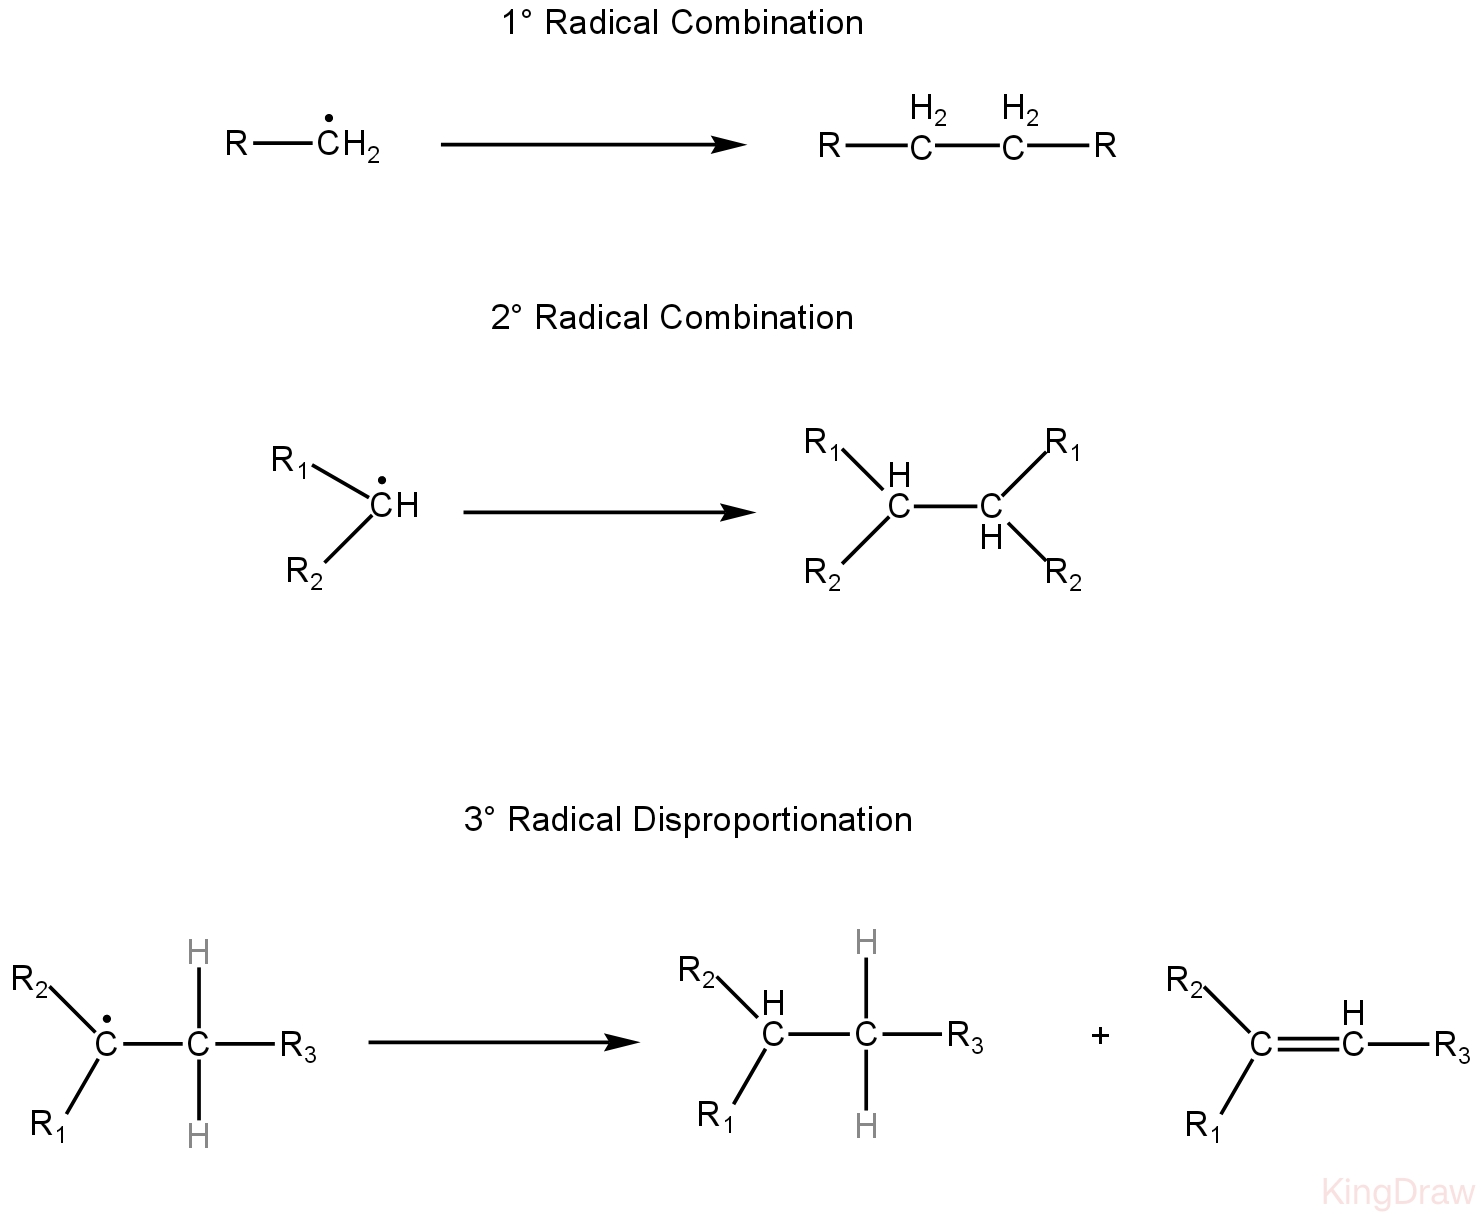
\includegraphics[scale=0.3]{FreeRadicalReaction(1)_1722161083701.JPEG}
\end{center}
\end{document}